\documentclass{standalone}
\usepackage{tikz}
\usetikzlibrary{patterns, positioning}
\usepackage[sfdefault]{ClearSans} %% option 'sfdefault' activates Clear Sans as the default text font
\usepackage[T1]{fontenc}

\begin{document}
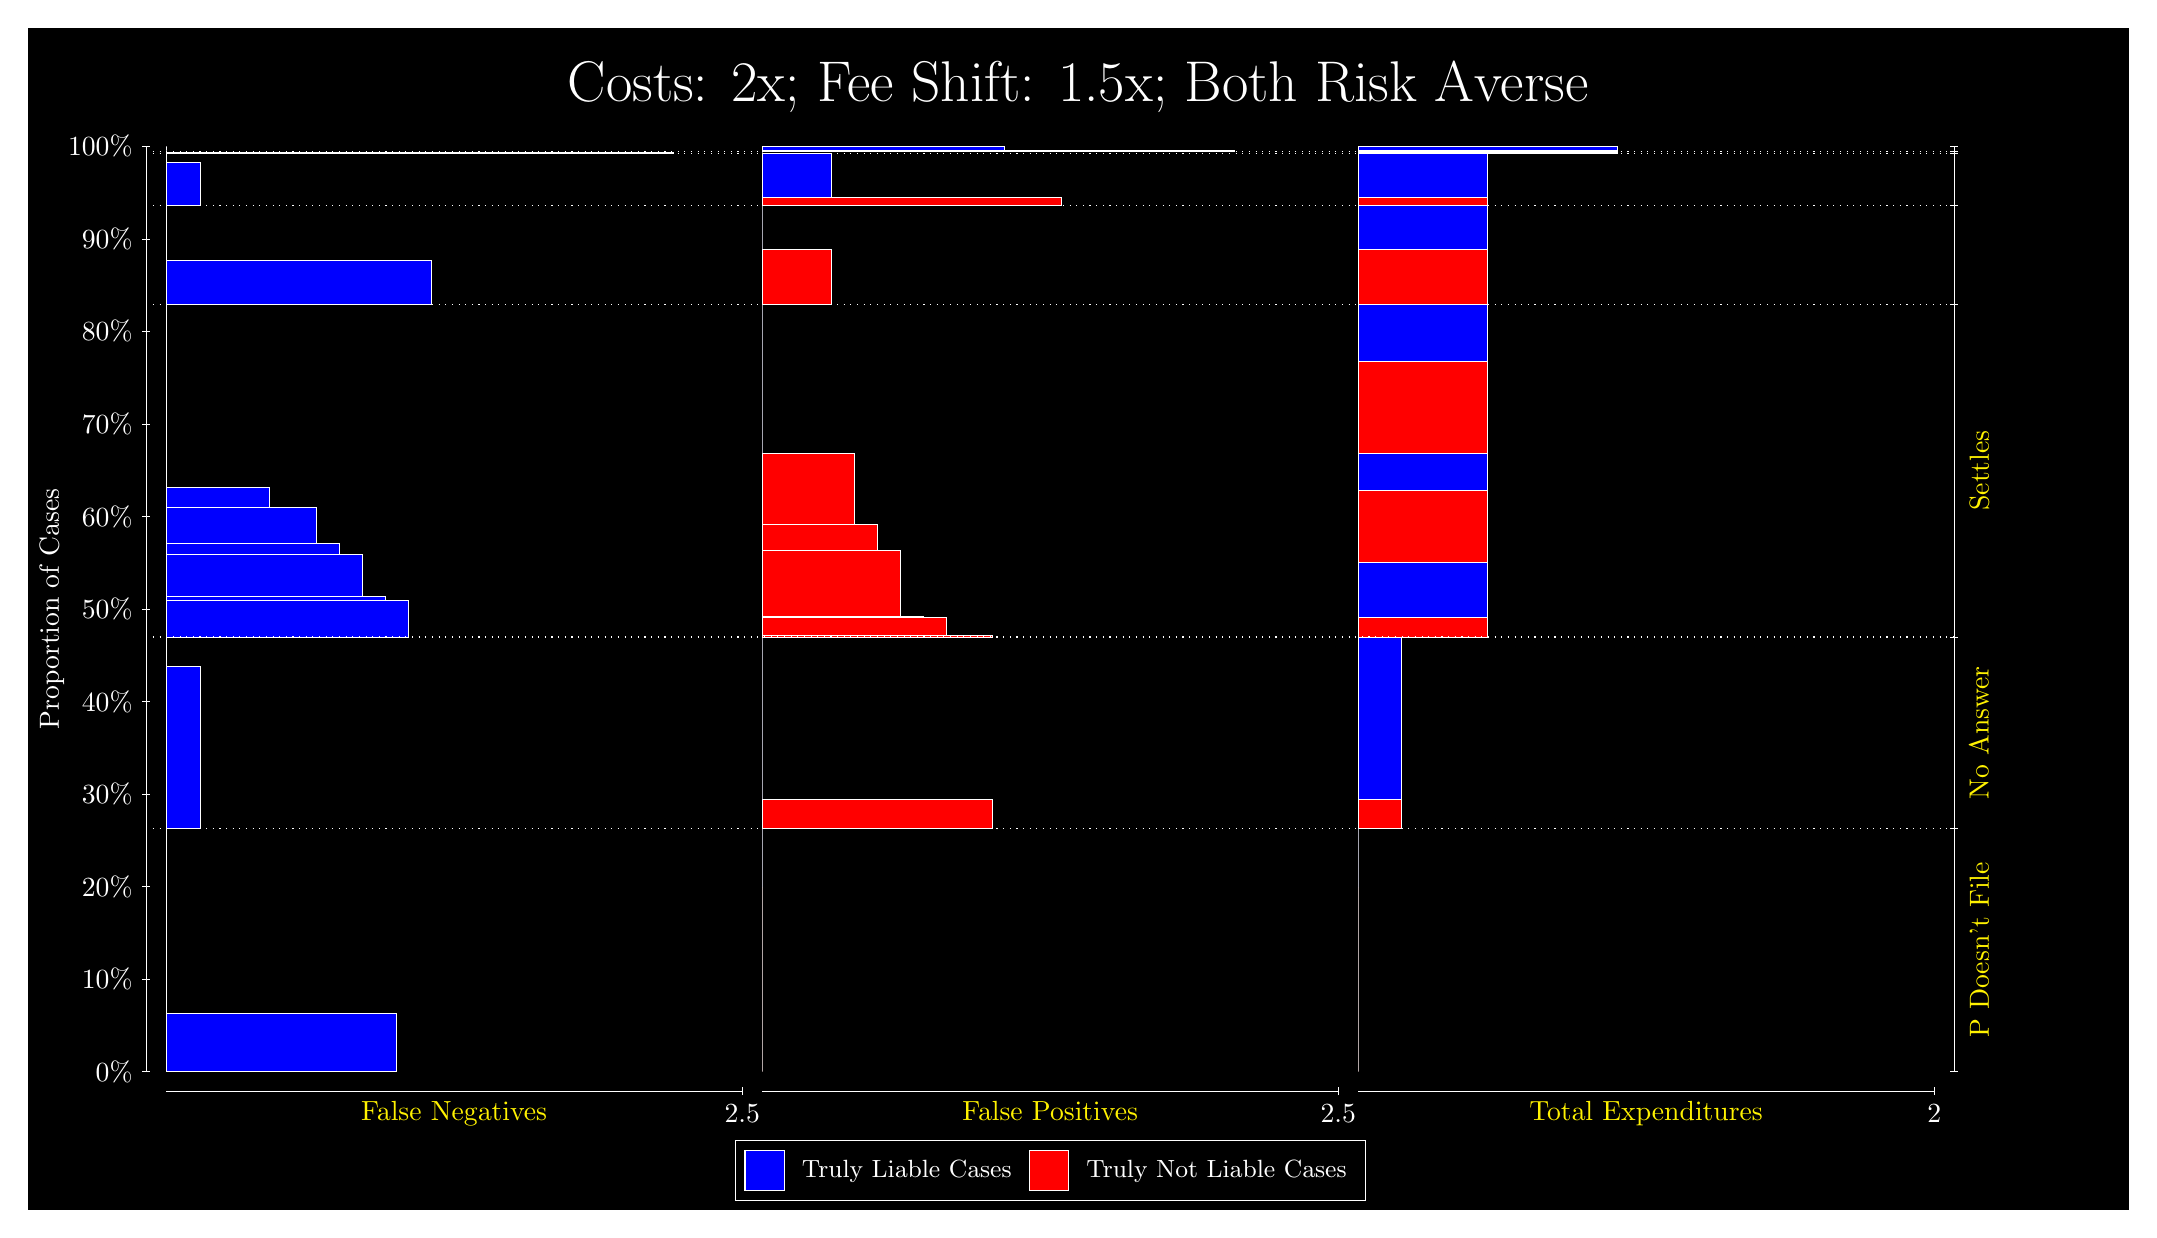
\begin{tikzpicture}
\draw[fill=black] (0,0) rectangle (26.667,15);
\draw[text=white] (0,13.5) rectangle (26.667,15) node[midway] {\huge Costs: 2x; Fee Shift: 1.5x; Both Risk Averse};
\draw[white, very thin] (1.5,1.75) -- (1.5,13.5);
\node[rotate=90, text=white, anchor=center] at (0.3, 7.625) {Proportion of Cases};
\draw[white, very thin] (1.45,1.75) -- (1.55,1.75);
\node[text=white, anchor=east] at (1.45, 1.75) {0\%};
\draw[white, very thin] (1.45,2.925) -- (1.55,2.925);
\node[text=white, anchor=east] at (1.45, 2.925) {10\%};
\draw[white, very thin] (1.45,4.1) -- (1.55,4.1);
\node[text=white, anchor=east] at (1.45, 4.1) {20\%};
\draw[white, very thin] (1.45,5.275) -- (1.55,5.275);
\node[text=white, anchor=east] at (1.45, 5.275) {30\%};
\draw[white, very thin] (1.45,6.45) -- (1.55,6.45);
\node[text=white, anchor=east] at (1.45, 6.45) {40\%};
\draw[white, very thin] (1.45,7.625) -- (1.55,7.625);
\node[text=white, anchor=east] at (1.45, 7.625) {50\%};
\draw[white, very thin] (1.45,8.8) -- (1.55,8.8);
\node[text=white, anchor=east] at (1.45, 8.8) {60\%};
\draw[white, very thin] (1.45,9.975) -- (1.55,9.975);
\node[text=white, anchor=east] at (1.45, 9.975) {70\%};
\draw[white, very thin] (1.45,11.15) -- (1.55,11.15);
\node[text=white, anchor=east] at (1.45, 11.15) {80\%};
\draw[white, very thin] (1.45,12.325) -- (1.55,12.325);
\node[text=white, anchor=east] at (1.45, 12.325) {90\%};
\draw[white, very thin] (1.45,13.5) -- (1.55,13.5);
\node[text=white, anchor=east] at (1.45, 13.5) {100\%};

\draw[white, very thin] (24.457,1.75) -- (24.457,13.5);
\draw[white, very thin] (24.407,1.75) -- (24.507,1.75);
\node[anchor=west] at (24.407, 1.75) {};
\draw[white, very thin] (24.407,4.8348) -- (24.507,4.8348);
\node[anchor=west] at (24.407, 4.8348) {};
\draw[white, very thin] (24.407,7.2686) -- (24.507,7.2686);
\node[anchor=west] at (24.407, 7.2686) {};
\draw[white, very thin] (24.407,11.495) -- (24.507,11.495);
\node[anchor=west] at (24.407, 11.495) {};
\draw[white, very thin] (24.407,12.747) -- (24.507,12.747);
\node[anchor=west] at (24.407, 12.747) {};
\draw[white, very thin] (24.407,13.41) -- (24.507,13.41);
\node[anchor=west] at (24.407, 13.41) {};
\draw[white, very thin] (24.407,13.435) -- (24.507,13.435);
\node[anchor=west] at (24.407, 13.435) {};
\draw[white, very thin] (24.407,13.5) -- (24.507,13.5);
\node[anchor=west] at (24.407, 13.5) {};

\draw[white, very thin, fill=blue] (1.75,1.75) rectangle (4.6775,2.493);
\draw[white, very thin, fill=red] (1.75,2.493) rectangle (1.75,4.8348);
\draw[white, very thin, fill=blue] (1.75,4.8348) rectangle (2.1891,6.8966);
\draw[white, very thin, fill=red] (1.75,6.8966) rectangle (1.75,7.2686);
\draw[white, very thin, fill=blue] (1.75,7.2686) rectangle (4.8239,7.7382);
\draw[white, very thin, fill=blue] (1.75,7.7382) rectangle (4.5312,7.7845);
\draw[white, very thin, fill=blue] (1.75,7.7845) rectangle (4.2384,8.3243);
\draw[white, very thin, fill=blue] (1.75,8.3243) rectangle (3.9457,8.4575);
\draw[white, very thin, fill=blue] (1.75,8.4575) rectangle (3.6529,8.9145);
\draw[white, very thin, fill=blue] (1.75,8.9145) rectangle (3.0674,9.1648);
\draw[white, very thin, fill=red] (1.75,9.1648) rectangle (1.75,11.495);
\draw[white, very thin, fill=blue] (1.75,11.495) rectangle (5.1167,12.049);
\draw[white, very thin, fill=red] (1.75,12.049) rectangle (1.75,12.747);
\draw[white, very thin, fill=blue] (1.75,12.747) rectangle (2.1891,13.303);
\draw[white, very thin, fill=red] (1.75,13.303) rectangle (1.75,13.41);
\draw[white, very thin, fill=blue] (1.75,13.41) rectangle (8.1906,13.422);
\draw[white, very thin, fill=red] (1.75,13.422) rectangle (1.75,13.435);
\draw[white, very thin, fill=red] (1.75,13.435) rectangle (1.75,13.447);
\draw[white, very thin, fill=blue] (1.75,13.447) rectangle (1.75,13.5);
\draw[white, very thin, fill=red] (9.3189,1.75) rectangle (9.3189,4.0918);
\draw[white, very thin, fill=blue] (9.3189,4.0918) rectangle (9.3189,4.8348);
\draw[white, very thin, fill=red] (9.3189,4.8348) rectangle (12.246,5.2068);
\draw[white, very thin, fill=blue] (9.3189,5.2068) rectangle (9.3189,7.2686);
\draw[white, very thin, fill=red] (9.3189,7.2686) rectangle (12.246,7.287);
\draw[white, very thin, fill=red] (9.3189,7.287) rectangle (11.661,7.5146);
\draw[white, very thin, fill=red] (9.3189,7.5146) rectangle (11.368,7.529);
\draw[white, very thin, fill=red] (9.3189,7.529) rectangle (11.075,8.3637);
\draw[white, very thin, fill=red] (9.3189,8.3637) rectangle (10.783,8.6939);
\draw[white, very thin, fill=red] (9.3189,8.6939) rectangle (10.49,9.5993);
\draw[white, very thin, fill=blue] (9.3189,9.5993) rectangle (9.3189,11.495);
\draw[white, very thin, fill=red] (9.3189,11.495) rectangle (10.197,12.193);
\draw[white, very thin, fill=blue] (9.3189,12.193) rectangle (9.3189,12.747);
\draw[white, very thin, fill=red] (9.3189,12.747) rectangle (13.125,12.854);
\draw[white, very thin, fill=blue] (9.3189,12.854) rectangle (10.197,13.41);
\draw[white, very thin, fill=red] (9.3189,13.41) rectangle (9.3189,13.423);
\draw[white, very thin, fill=blue] (9.3189,13.423) rectangle (9.3189,13.435);
\draw[white, very thin, fill=red] (9.3189,13.435) rectangle (15.32,13.447);
\draw[white, very thin, fill=blue] (9.3189,13.447) rectangle (12.393,13.5);
\draw[white, very thin, fill=red] (16.888,1.75) rectangle (16.888,4.0918);
\draw[white, very thin, fill=blue] (16.888,4.0918) rectangle (16.888,4.8348);
\draw[white, very thin, fill=red] (16.888,4.8348) rectangle (17.437,5.2068);
\draw[white, very thin, fill=blue] (16.888,5.2068) rectangle (17.437,7.2686);
\draw[white, very thin, fill=red] (16.888,7.2686) rectangle (18.534,7.5146);
\draw[white, very thin, fill=blue] (16.888,7.5146) rectangle (18.534,8.2219);
\draw[white, very thin, fill=red] (16.888,8.2219) rectangle (18.534,9.1273);
\draw[white, very thin, fill=blue] (16.888,9.1273) rectangle (18.534,9.5969);
\draw[white, very thin, fill=red] (16.888,9.5969) rectangle (18.534,10.776);
\draw[white, very thin, fill=blue] (16.888,10.776) rectangle (18.534,11.495);
\draw[white, very thin, fill=red] (16.888,11.495) rectangle (18.534,12.193);
\draw[white, very thin, fill=blue] (16.888,12.193) rectangle (18.534,12.747);
\draw[white, very thin, fill=red] (16.888,12.747) rectangle (18.534,12.854);
\draw[white, very thin, fill=blue] (16.888,12.854) rectangle (18.534,13.41);
\draw[white, very thin, fill=red] (16.888,13.41) rectangle (20.181,13.423);
\draw[white, very thin, fill=blue] (16.888,13.423) rectangle (20.181,13.435);
\draw[white, very thin, fill=red] (16.888,13.435) rectangle (20.181,13.447);
\draw[white, very thin, fill=blue] (16.888,13.447) rectangle (20.181,13.5);
\draw[white, dotted] (1.5,4.8348) -- (24.457,4.8348);
\draw[white, dotted] (1.5,7.2686) -- (24.457,7.2686);
\draw[white, dotted] (1.5,11.495) -- (24.457,11.495);
\draw[white, dotted] (1.5,12.747) -- (24.457,12.747);
\draw[white, dotted] (1.5,13.41) -- (24.457,13.41);
\draw[white, dotted] (1.5,13.435) -- (24.457,13.435);
\draw[white, very thin] (1.75,1.5) -- (9.0689,1.5);
\node[text=yellow, anchor=north] at (5.4094, 1.5) {False Negatives};
\draw[white, very thin] (9.0689,1.45) -- (9.0689,1.55);
\node[text=white, anchor=north] at (9.0689, 1.45) {2.5};

\draw[white, very thin] (9.3189,1.5) -- (16.638,1.5);
\node[text=yellow, anchor=north] at (12.978, 1.5) {False Positives};
\draw[white, very thin] (16.638,1.45) -- (16.638,1.55);
\node[text=white, anchor=north] at (16.638, 1.45) {2.5};

\draw[white, very thin] (16.888,1.5) -- (24.207,1.5);
\node[text=yellow, anchor=north] at (20.547, 1.5) {Total Expenditures};
\draw[white, very thin] (24.207,1.45) -- (24.207,1.55);
\node[text=white, anchor=north] at (24.207, 1.45) {2};

\node[text=yellow, centered, rotate=90] at (24.777, 3.2924) {P Doesn't File};
\node[text=yellow, centered, rotate=90] at (24.777, 6.0517) {No Answer};
\node[text=yellow, centered, rotate=90] at (24.777, 9.382) {Settles};





\draw (12.978300999999998,1.5) node[draw=none] (baseCoordinate) {};
\begin{scope}[align=center]
        \matrix[scale=0.5, draw=white, below=0.5cm of baseCoordinate, nodes={draw}, column sep=0.1cm]{
            \node[rectangle, draw, minimum width=0.5cm, minimum height=0.5cm, fill=blue] {}; &
            \node[draw=none, font=\small, text=white] (B) {Truly Liable Cases}; &
            \node[rectangle, draw, minimum width=0.5cm, minimum height=0.5cm, fill=red] {}; &
            \node[draw=none, font=\small, text=white] (B) {Truly Not Liable Cases}; \\
            };
\end{scope}

\end{tikzpicture}
\end{document}